%\let\textcircled=\pgftextcircled
\chapter{Introduction}
\label{chap:intro}

\textbf{Vehicle dynamics reconstruction} is a topic with much interest especially in insurance makers. A car crash can be recreated visually after the event happened. But there are other topics with interest in vehicle dynamics reconstruction, like self-driving vehicles or everything interested in knowing the vehicle position at some point in time. \\
This thesis will analyze techniques for reconstruction based on inertial and GNSS data used in a related software project. \\
In the data collected and used for the project:
\begin{itemize}
\item \textbf{inertial} data was created by accelerometers and gyroscopes, which measures respectively linear accelerations and angular velocities in a local reference frame. 
\item \textbf{GNSS} (Global Navigation Satellite System) was created by an eletronic receiver. GNSS receivers provide latitudes, longitudes and alititudes. One of the most famous GNSS is the american GPS (Global Positioning System) but during experiments also russian GLONASS and chinese BeiDou signals were received. 
\end{itemize}
All these sensors can be bundled in a box, as in our case, and fitted on a vehicle. \\


\begin{figure}[H]
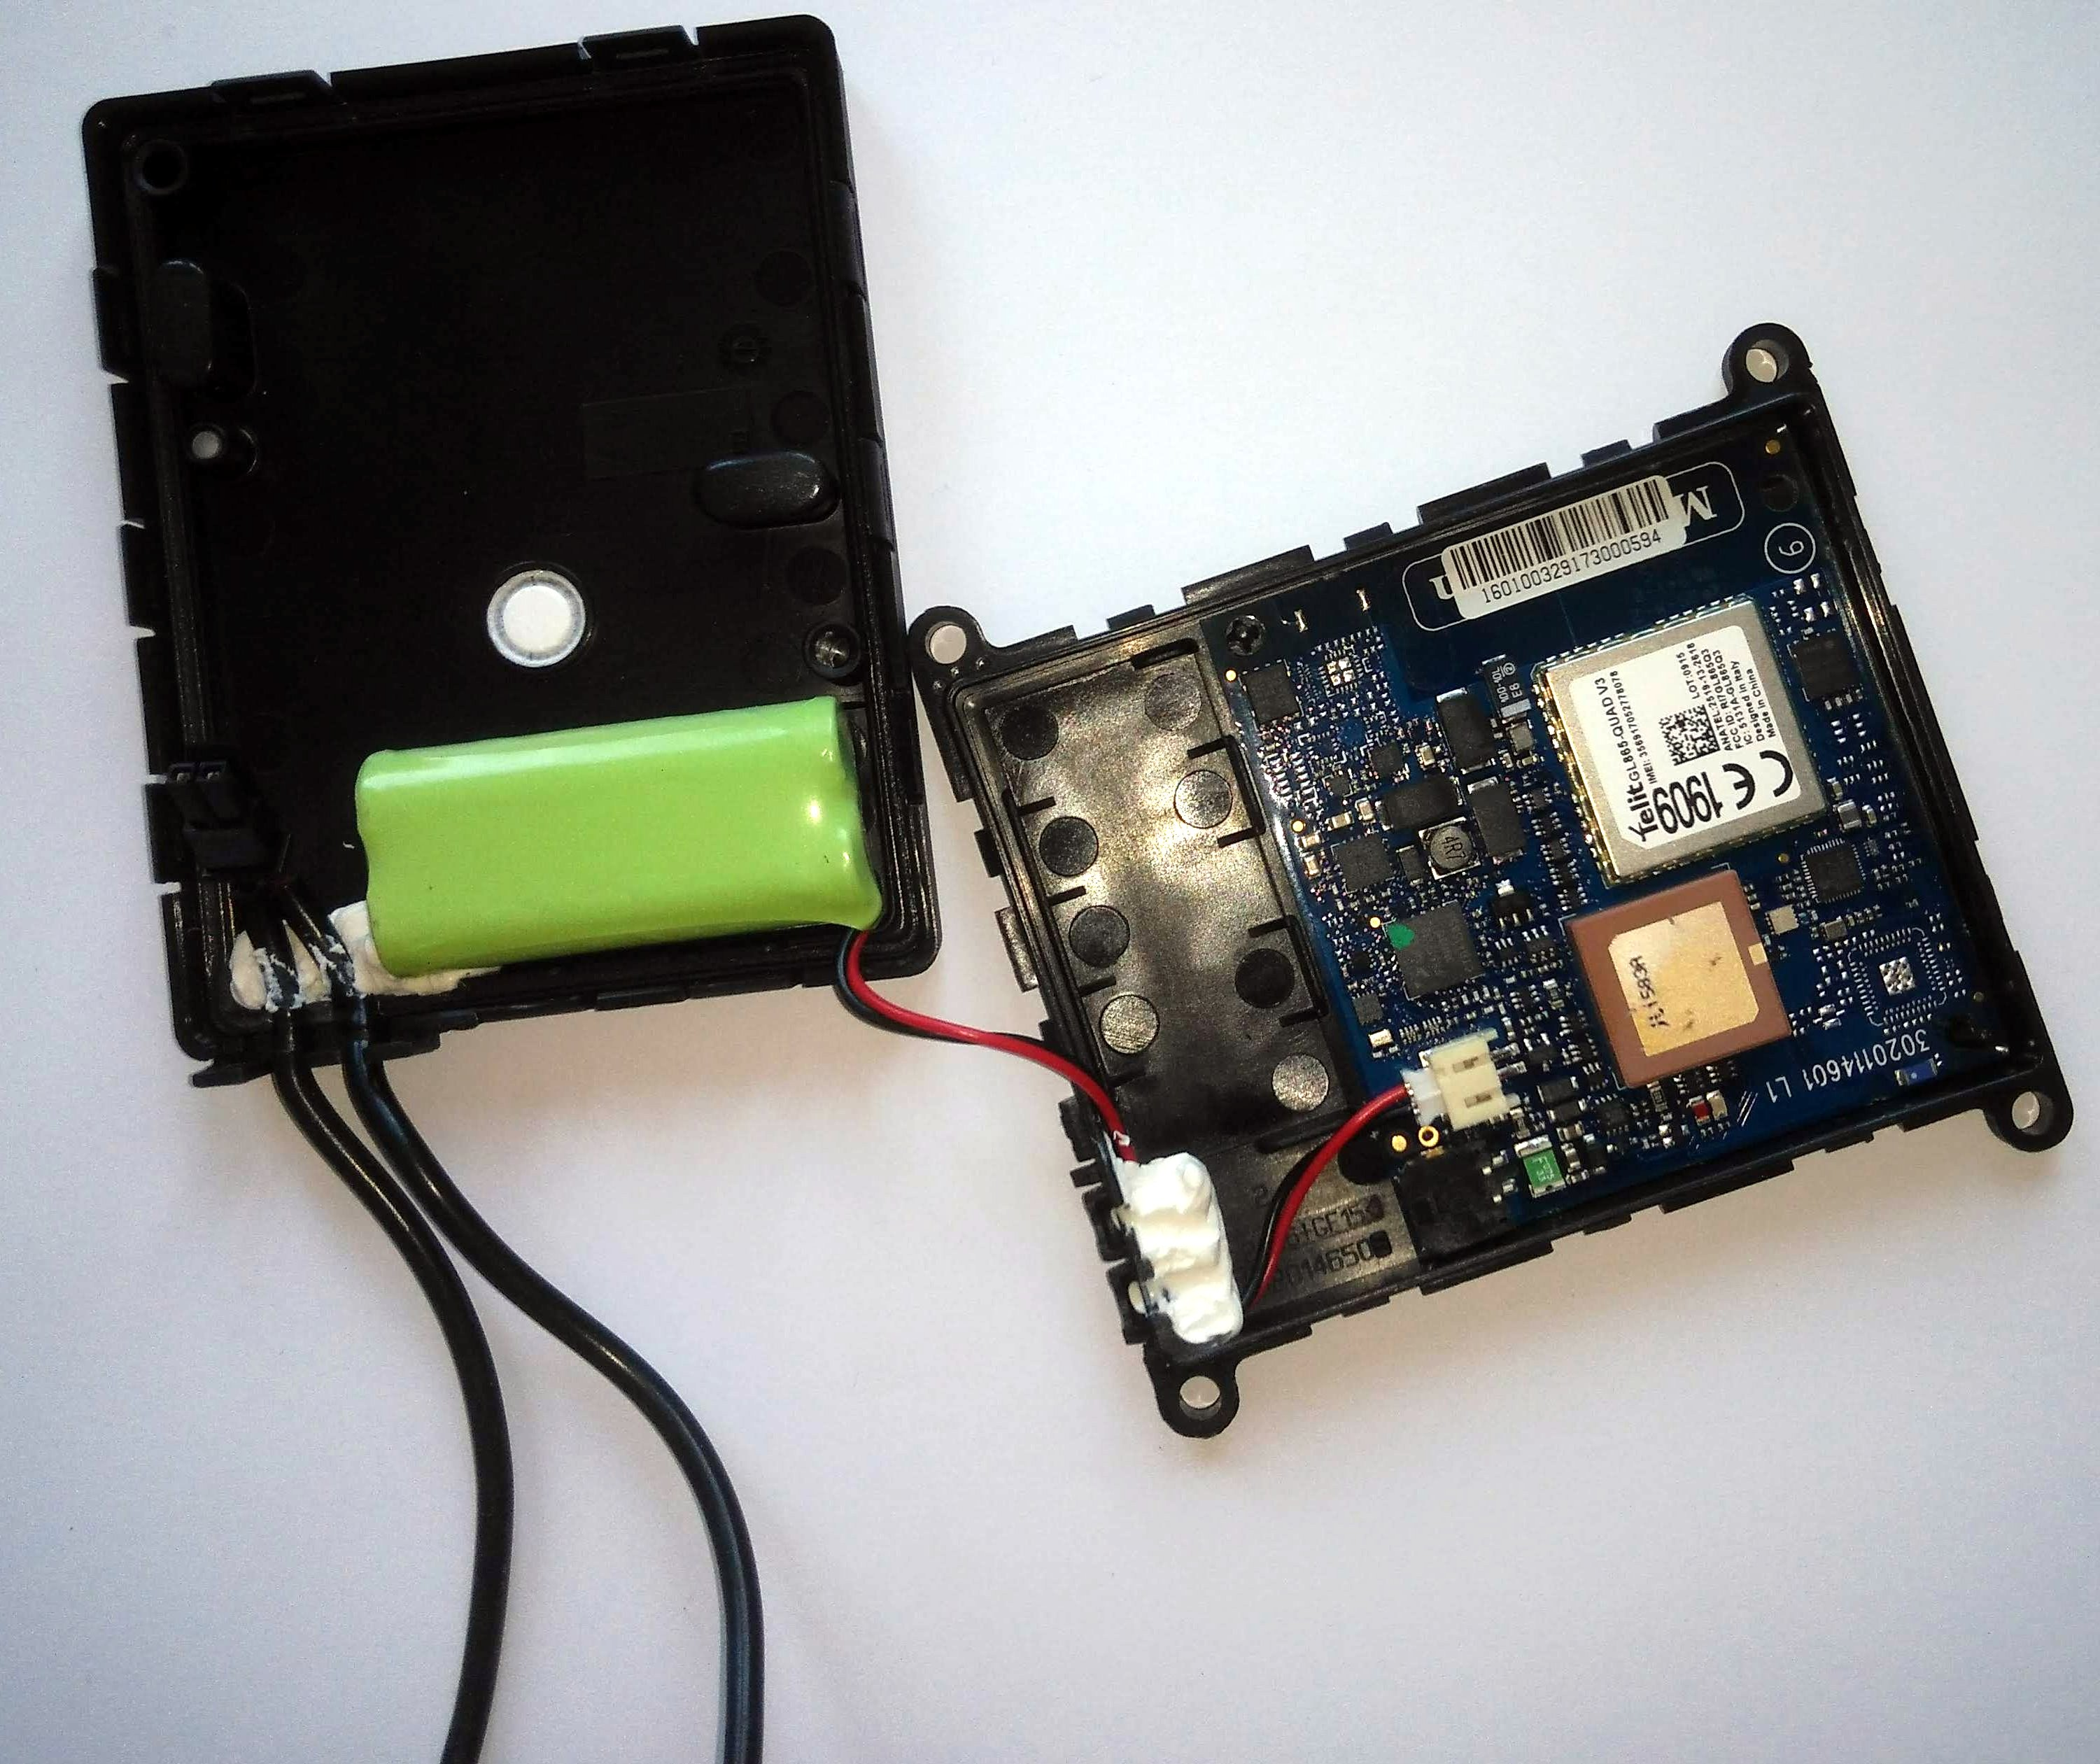
\includegraphics[width=\linewidth]{box.jpg}
\caption{One of the sensor box used to collect data}
\end{figure}

\begin{flushleft}

The experiment will consist of verifying the possibility of creating a software capable of recreating a vehicle dynamic visually realistic.
The validation of results will be, in a first initial phase where effectiveness of the program will be low, exclusively visually empiric, because of the need of rapid development and testing times. In a second and later phase, when quality of output will become more difficult to evaluate empirically, result will be compared to picture and video footage captured in the data acquisition phase. \\

Challenges the aspiring software solution may face are: sensor data gathering and transmission, correction of bad alignment of sensors, integration numerical error, precision reinforcement with multiple sensor fusion, representation of reconstructed trajectory. \\

Input date format is specified in a Physycom Github oline repository available in \href{https://github.com/physycom/file_format_specifications/blob/master/formati_file.md}{this url}. I searched for an universal standard file format for inertial and GSSS data but i didn't find previous works. \\
Briefly formats supported by the software are all the following combination:
\end{flushleft}

\begin{center}
\begin{table}[H]
\begin{tabular}{l|l|l|}
\cline{2-3}
 & \textbf{inertial} & \textbf{inertial+GNSS} \\ \hline
\multicolumn{1}{|l|}{\textbf{interpolated}} & inertial & fullinertial \\ \hline
\multicolumn{1}{|l|}{\textbf{non interpolated}} & unmodified-inertial & unmodified-fullinertial \\ \hline
\end{tabular}
\end{table}

\end{center}


\begin{flushleft}
\textit{full-inertial} format is the more complete, it contains both accelerometer, gyroscope and GNSS data. Indeed, the program will give a better output when provided with a \textit{full-inertial} input file, as it have more data to improve reconstruction. 
Records data can be interpolated, in this case records have always data from all sensors, instead of only from inertial sensor or GNSS sensor, as they have different frequencies. \\
In the case input data isn't interpolated, the software will take care of doing it. \\

The following table shows \textit{full-inertial} data format in the order is present in the input files.

\begin{table}[H]
\begin{tabular}{|c|c|c|c|c|}
\hline
\begin{tabular}[c]{@{}c@{}}Dataset\\ Column\\ Index\end{tabular} & Name & Type & \begin{tabular}[c]{@{}c@{}}Unit\\ of\\ measure\end{tabular} & Notes \\ \hline
0 & Timestamp & Float & Seconds & From 1/1/2000 UTC+1 \\ \hline
1 & Latitude & Float & Degrees & From -90 to +90 \\ \hline
2 & Longitude & Float & Degrees & From -180 to +180 \\ \hline
3 & Altitude & Float & Meters & from sea level \\ \hline
4 & Heading & Float & Degrees & \begin{tabular}[c]{@{}c@{}}Measured from magnetic\\ north, from 0 to 360\end{tabular} \\ \hline
5 & Speed & Float & Km/h &  \\ \hline
6 & Acceleration X & Float & g-unit & Inertial \\ \hline
7 & Acceleration Y & Float & g-unit & Inertial \\ \hline
8 & Acceleration Z & Float & g-unit & Inertial \\ \hline
9 & Angular speed X & Float & Degrees/Seconds & \begin{tabular}[c]{@{}c@{}}right-handed \\ reference system\end{tabular} \\ \hline
10 & Angular speed Y & Float & Degrees/Seconds & \begin{tabular}[c]{@{}c@{}}right-handed \\ reference system\end{tabular} \\ \hline
11 & Angular speed Z & Float & Degrees/Seconds & \begin{tabular}[c]{@{}c@{}}right-handed \\ reference system\end{tabular} \\ \hline
12 & Acceleration module & Float & g-unit &  \\ \hline
13 & Relative time & Float & Seconds & From first record \\ \hline
\end{tabular}
\end{table}

Lastly, I decided to visualize the reconstructed trajectory animated on the 3D modeling software Blender. The decision is motivated by the fact that Blender is a popular open source software and have an API to interact with, additionally it's already used inside the research group and one of its member is a 3d-artist specialized on it.
%TODO talk abot blender popularity with google trends as source?
\end{flushleft}